\chapter{TLS in der Lehre}
\label{cha_tls_teaching}

In diesem Abschnitt soll darauf eingegangen werden, warum sich die Beschäftigung mit TLS in der Hochschullehre im Bereich der IT-Sicherheit anbietet. %Darauffolgend werden einige Schwerpunkte herausgearbeitet, die sich für die Lehre anbieten, und anschließend mit explorativen Lernen auf eine Methode eingegangen, die für das Verstehen von TLS hilfreich sein kann.

In Abschnitt \ref{sec_tls_overview} wurde bereits die Bedeutung und umfassende Verwendung von TLS erwähnt. Dies ist ein Grund dafür, dass jeder, der sich detaillierter mit IT-Sicherheit beschäftigt, auch die Grundlagen von TLS verstehen sollte. Auch viele Angriffe, die gegen TLS entwickelt wurden, und die entsprechenden Gegenmaßnahmen bieten gute Möglichkeiten, um sie in der Lehre einzusetzen. Je nach gewünschten Schwerpunkten lassen sich beispielsweise Angriffe im Bereich der Kryptographie oder der Protokollspezifikation nutzen. Sogar eine Betrachtung des gesellschaftlichen bzw. politischen Kontexts bietet sich an\footnote{Die Vorschrift für die Bereitstellung von exportgeschwächten \ciphersuites{} durch die US-Regierung könnte hier beispielsweise ein Ausgangspunkt sein.}. \\
Zusätzlich spricht für einen Einsatz in der Lehre auch die ebenfalls bereits erwähnte einfache Protokollspezifikation, durch die der Blick auf wesentliche Prinzipien der IT-Sicherheit erleichtert wird. Auf einige dieser Prinzipien soll im nächsten Abschnitt eingegangen werden.

\section{Schwerpunkte für die Lehre}

In \cite{schubert11} wird das didaktische Prinzip nach J. S. Brunner erwähnt, wonach die Lehre sich \inquotes{in erster Linie an den Strukturen der zugrundeliegenden Wissenschaft orientieren soll}. Diese Strukturen werden auch Fundamentale Ideen genannt.

Hierbei handelt es sich um \inquotes{langlebige Konzepte}, die die \inquotes{Übertragung (Transfer) früher erworbener Kenntnisse auf [neue] Situationen} \cite{schubert11} ermöglichen sollen. Insbesondere der  sollte den Autoren zufolge an allgemeinbildenden Schulen und in der Hochschullehre im Vordergrund stehen. Dieser nicht\-spe\-zi\-fische Transfer beschreibt das Lernen von grundlegenden Begriffen, Prinzipien und Denkweisen - im Gegensatz zum spezifischen Transfer, dem geringfügigen Anpassen einer Situation an die Lösung eines ähnlichen, bekannten Problems.

Kennzeichnend für Fundamentale Ideen sind unter anderem das Horizontal- und das Zeitkriterium, also die umfassende Anwendbarkeit oder Erkennbarkeit in vielen Bereichen einer Wissenschaft und ebenso die längerfristige Relevanz der Idee. 

Als Empfehlung für die Hochschuldidaktik fassen die Autoren dieses Prinzip folgendermaßen zusammen:

\begin{quote}
\inquotes{Jeder Student wird im Laufe seines Berufslebens vermutlich mehreren Paradigmenwechseln der Informatik gegenüberstehen, wobei jeweils ein größerer Teil seines Wissens überflüssig oder fehlerhaft wird. Daher sollten die Fähigkeiten, die er während des Studiums erwirbt, möglichst robust gegenüber neuen wissenschaftlichen Entwicklungen sein und ihn befähigen,  Paradigmenwechsel  zu  bewältigen.  Folglich  müssen  Studenten  ein Bild von den dauerhaften Grundlagen, den Fundamentalen Ideen, Prinzipien, Methoden und Denkweisen der Informatik erlangen. Dazu sind in Vorlesungen und  Lehrbüchern  stets  die  Fundamentalen  Ideen,  die  sich  hinter  den  jeweils 
behandelten Sachgebieten verbergen, herauszuarbeiten, zu betonen, zu anderen Teilgebieten in Beziehung zu setzen und so in einen übergeordneten Zusammenhang  einzuordnen.} \cite{schubert11}
\end{quote}

Auch wenn das Prinzip Fundamentaler Ideen umfassender ist als das eingeschränkte Thema dieser Arbeit, so lässt sich doch eine klare Empfehlung für die Betrachtung von TLS (oder anderer konkreter Protokolle oder Verfahren) in der Hochschullehre ableiten. Es sollten  insbesondere Prinzipien betrachtet werden, die als häufig verwendet und auch langfristig gültig für den Bereich der IT-Sicherheit, der Kryptographie oder der Sicherheitsprotokolle angesehen werden können. 
Dieses Vorgehen wird auch von Klüver und Klüver als zentrale Aufgabe der Didaktik ausgemacht und als didaktische Reduktion, also \inquotes{die Rückführung komplexer Sachverhalte auf ihre wesentlichen  Elemente,  um  sie  für  Lernende  überschaubar  und  begreiflich  zu  machen} \cite{kluever12}, bezeichnet.

Im Folgenden sollen einige Vorschläge für solche Prinzipien aufgeführt werden, deren Bedeutung durch Angabe weiterer Bereiche, in denen sie zur Anwendung kommen, deutlich wird. 

\subsection{Hybride Kryptosysteme}

In Kapitel \ref{cha_cryptographic_techniques} wurde bereits auf das Problem des Schlüsselaustausches bei symmetrischen Algorithmen zur Ver- und Entschlüsselung eingegangen. Durch asymmetrische Verfahren lässt sich dieses Problem leicht lösen. Diese benötigen jedoch deutlich mehr Zeit für die Verarbeitung von Daten als symmetrische Verfahren. 

Um die Vorteile beider Lösungen zu kombinieren, werden häufig hybride Kryptosysteme eingesetzt: Es wird für jede neue Kommunikation ein symmetrischer Schlüssel zufällig generiert (daher Sitzungsschlüssel genannt) und dem Kommunikationspartner mit dessen öffentlichem Schlüssel verschlüsselt zugesendet. Eine andere Möglichkeit ist die Schlüsselvereinbarung per Diffie-Hellman-Verfahren (vgl. Abschnitt \ref{sec_diffie_hellman}). Nach der Entschlüsselung oder Vereinbarung sind beide Partner im Besitz des gleichen Sitzungsschlüssels und können ihre Kommunikation symmetrisch verschlüsseln \cite{Schneier2006}.

Dieses Prinzip kommt neben seiner Anwendung in TLS unter anderem auch in IPSec und PGP zum Einsatz.

\subsection{Problem des Schlüsselaustausches und Authentifizierung}

Wie ebenfalls bereits in Kapitel \ref{cha_cryptographic_techniques} erwähnt, besteht bei der Nutzung von asymmetrischen Verfahren jedoch das Problem, die Identität des Besitzers des öffentlichen Schlüssels sicherzustellen.

Dieses Problem soll kurz erläutert werden. Möchte eine Person A eine Nachricht asymmetrisch verschlüsselt mit B austauschen, so benötigt sie den öffentlichen Schlüssel \(K^B_\text{public}\) von B. Ein Angreifer M, der die Kommunikation zwischen A und B lesen und verändern kann (ein sogenannter Man-in-the-Middle), kann diesen öffentlichen Schlüssel bei der Übermittlung durch seinen eigenen \(K^M_\text{public}\) austauschen. Die Nachricht von A kann er nun mit seinem geheimen Schlüssel entschlüsseln. Damit sein Angriff unbemerkt bleibt, kann er die Nachricht anschließend noch mit \(K^B_\text{public}\) verschlüsseln und an B senden. Dieser Angriff ist in Abbildung \ref{fig_mitm} dargestellt.

\begin{figure}
	\centering
	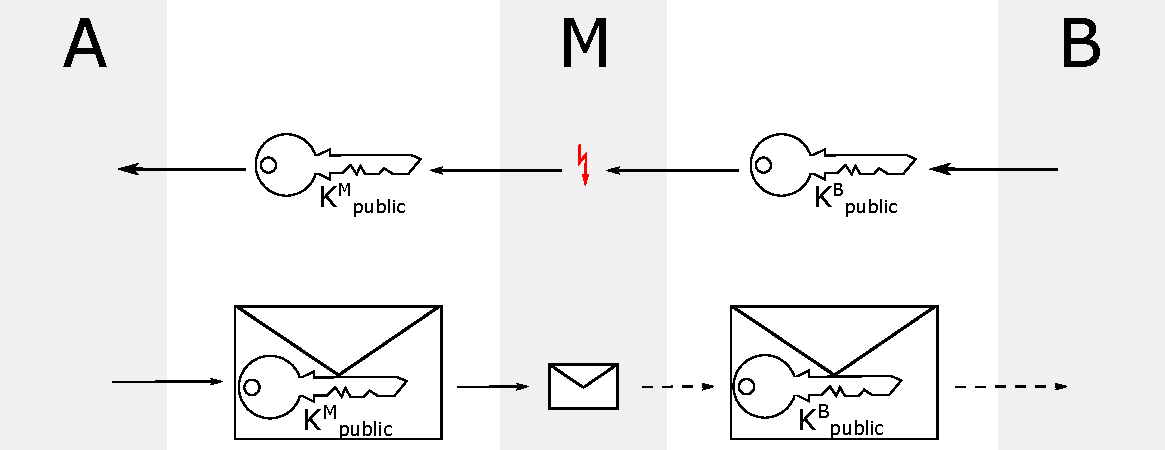
\includegraphics[width=15cm]{Diagrams/mitm.pdf} %
	\caption{Man-in-the-middle-Angriff auf den Schlüsselaustausch}
	\label{fig_mitm}
\end{figure}

Um diesen Angriff zu verhindern, muss es eine Möglichkeit geben, den Besitzer des Schlüssels zu verifizieren. Für diese Aufgabe wird in SSL/TLS auf Zertifikate und eine Public-Key-Infrastruktur (PKI) gesetzt. Ein Zertifikat enthält den öffentlichen Schlüssel und die Informationen des Besitzers - bestehend aus dem Namen oder der URL des Servers und weiteren Angaben. Dieses Zertifikat wird von einer vertrauenswürdigen Instanz, der Certificate Authority (CA), nach der Überprüfung der Besitzeridentität mit ihrem geheimen Schlüssel signiert. Ein Empfänger des Zertifikats kann nun das Zertifikat mit dem öffentlichen Schlüssel der CA überprüfen, in dessen Besitz er im Vorwege sein muss\footnote{
	Heutige Browser und Betriebssysteme werden bereits mit Listen solcher CAs ausgeliefert.
}. Danach sind der Besitzer und der zugehörige öffentliche Schlüssel verifiziert und der Schlüssel kann zum Verschlüsseln von Nachrichten genutzt werden\footnote{
	Die Schwächen, die in diesem System bestehen können, sind vielfältig, liegen jedoch nicht im Fokus dieser Arbeit. Erste Hinweise sind in Abschnitt \ref{sec_certificates} und in \cite{ferguson10} zu finden.
}. 

Die Nutzung von Zertifikaten und PKIs findet unter anderem auch in IPSec oder S/MIME Verwendung. 

\subsection{Seitenkanalangriffe}
Seitenkanalangriffe sind Angriffe, die nicht das kryptographische Verfahren direkt angreifen, sondern versuchen, Informationen über die Nachricht oder verwendete Schlüssel aus anderen Kanälen zu erhalten. Hierbei kann es sich beispielsweise um Zeit- oder Stromverbrauchsmessung handeln, aber auch um die Messung der elektromagnetischen Abstrahlung, des Schalls oder sogar des Erdungspotentials eines Rechners. 

Wenn sich unterschiedliche Schlüssel- oder Nachrichtenbits verschieden auf die Werte des Seitenkanals auswirken, so lassen sich Schlüssel bzw. Nachricht oftmals aus den gemessenen Informationen ableiten. Gerade bei einfachen Geräten wie Smartcards können schon einfache Angriffe erfolgreich sein.

Um vor Seitenkanalangriffen geschützt zu sein, muss eine Implementierung sich für unterschiedliche Eingaben möglichst gleich verhalten. Als Maßnahme gegen Timing-Angriffe (also die Messung der benötigten Zeit für eine Operation) ist beispielsweise die Einführung einer konstanten Zeit für die Ausführungsdauer möglich. Dazu wird eine Zeit \(d\) gewählt, die länger ist als jede mögliche benötigte Ausführungsdauer \(t\) der Operation. Nach der Ausführung wird immer der Zeitraum \(d-t\) abgewartet, sodass die Operation insgesamt die konstante Zeit \(d\) benötigt.\\
Diese Möglichkeit schützt natürlich nicht vor anderen Seitenkanalangriffen, für deren Abwehr andere Schutzmaßnahmen getroffen werden müssen \cite{ferguson10}.

Seitenkanalangriffe in Form von Timing-Angriffen werden auch bei einigen Angriffen gegen SSL/TLS eingesetzt, wie beispielsweise bei dem Bleichenbacher- (Abschnitt \ref{sec_attack_bleichenbacher}) oder dem Padding-Orakel-Angriff (Abschnitt \ref{sec_attack_padding_oracle}).

\subsection{Replay-Angriffe}

Bei einem Replay-Angriff sendet ein Angreifer zuvor aufgenommene Nachrichten erneut an den Empfänger. Da es sich um eine echte Nachricht handelt, müssen Gegenmaßnahmen getroffen werden, um dieses erneute Senden zu erkennen. Möglichkeiten hierfür sind beispielsweise die Einführung von Sequenznummern wie bei TLS, die Nutzung von Zeitstempeln oder ein Challenge-Response-Verfahren, das einem Sender eine zufällige Aufgabe stellt, deren Lösung er in der Nachricht mitsenden muss \cite{ferguson10}.

Die Abwehr von Replay-Angriffen muss in allen Sicherheitsprotokollen bedacht werden.

\subsection{Kryptographische Prinzipien}
\label{sec_didactics_crypto}

%Zufällige IVs in CBC, MAC-then-encrypt, AEAD(?)

TLS bietet auch Beispiele für grundlegende Prinzipien, die bei der Verwendung von kryptographischen Verfahren zu beachten sind. Auf zwei dieser Beispiele soll genauer eingegangen werden.

Ein Prinzip betrifft die Reihenfolge, in der Verschlüsselung und Authentifizierung einer Nachricht stattfinden. 
In TLS wird bei Nutzung von Block- und Stream-\ciphersuites{} für eine Nachricht zuerst ein MAC berechnet, der anschließend zusammen mit der Nachricht verschlüsselt wird. Diese Reihenfolge der Operationen wird MAC-then-Encrypt genannt. \\
Laut \cite{AE2000} ist Encrypt-then-MAC vorzuziehen. In \cite{krawczyk01} wird dieses Ergebnis bestätigt, aber auch die Sicherheit von MAC-then-Encrypt unter bestimmten Voraussetzungen gezeigt.\\
In \cite{ferguson10} fügen die Autoren hinzu, dass das Erkennen und Verwerfen ungültiger Nachrichten durch Encrypt-then-MAC vereinfacht wird. Auf der anderen Seite werden aber auch Vorteile der MAC-then-Encrypt-Reihenfolge erwähnt: Die Ein- und Ausgabe der MAC-Funktion sind einem Angreifer verborgen, so dass Angriffe gegen den MAC erschwert werden und die Integrität der Nachricht damit besser geschützt ist. Außerdem wird auf das Horton-Prinzip hingewiesen: \inquotes{Authenticate what is meant, not what is said} \cite{wagner96}. Es sollte also grundsätzlich die ursprüngliche Bedeutung einer Nachricht und nicht eine eventuelle Transformation der Nachricht (beispielsweise Verschlüsselung) authentifiziert werden.\\
In den meisten Veröffentlichungen wird jedoch die Nutzung von Encrypt-then-MAC gefordert \footnote{
	Siehe beispielsweise auch Moxie Marlinspike: The Cryptographic Doom Principle. \\
	http://www.thoughtcrime.org/ blog/ the-cryptographic-doom-principle/ Abgerufen am 15.10.2015.
}. In TLS hätte die Verwendung dieser Reihenfolge beispielsweise den Padding-Orakel-Angriff (siehe Abschnitt \ref{sec_attack_padding_oracle}) verhindert. Auch die Nutzung von AEAD-Chiffren verhindert Probleme mit dieser Reihenfolge, da die Authentizität einer Nachricht bereits durch die Chiffre gewährleistet wird.

Ein weiteres Prinzip ist die Nutzung unvorhersagbarer Initialisierungsvektoren für Blockchiffren im CBC-Modus, die beispielsweise in \cite{ferguson10} von den Autoren gefordert wird. In TLS 1.0 wurde der letzte Chiffretextblock als IV genutzt, was den in Abschnitt \ref{sec_known_ivs} beschriebenen Angriff ermöglichte.

Diese Prinzipien sind nicht TLS-spezifisch, sondern sollten in allen Fällen beachtet werden, in denen Kryptographie eingesetzt wird.

\section{Lernen durch Exploration}
\label{sec_exploration}

Wie im letzten Abschnitt exemplarisch deutlich wurde, eignet sich TLS aus vielerlei Gründen für den Einsatz in der Hochschullehre.\\
Eine spezielle Methode, die in der Lehre zum Einsatz kommen kann und mit der sich diese Arbeit beschäftigen wird, ist die Exploration.

Exploratives Lernen, also \inquotes{entdeckendes, forschendes oder autonomes Lernen}, empfiehlt sich für Bereiche, deren \inquotes{Abstraktion oder Komplexität mit anderen Lernmaterialien schwerer erfassbar oder schwerer darstellbar [ist]} \cite{schubert11}. 
Allerdings wird geeignete Software (Explorationsmodule bzw. lernförderliche Software) benötigt, die den Lernenden beim explorativen Lernen unterstützt. Hierfür bieten sich oftmals Simulationen an. 

\begin{quote}
\inquotes{Simulationen sind Computerprogramme, die Phänomene oder Aktivitäten modellieren und die dafür vorgesehen sind, dass die Nutzer durch Interaktionen mit ihnen etwas über diese Phänomene und Aktivitäten lernen.} \cite{niegemann08}
\end{quote}

Sie ermöglichen es, mit dem Lernstoff zu interagieren, und Prozesse, die normalerweise nicht beobachtbar sind, sichtbar und erfahrbar zu machen. Durch die Manipulation von dynamischen Elementen können Lernende die Auswirkungen auf das Verhalten eines Systems direkt beobachten \cite{niegemann08}.

Für erfolgreich zu verwendende Simulationen ist es nötig, Lernenden die Sicht sowohl auf sichtbare als auch auf  nicht sichtbare Konzepte und Komponenten, die in einem System verwendet werden, zu ermöglichen. Dazu ist es immer erforderlich, verborgen ablaufende Prozesse an die Benutzeroberfläche der Simulation zu bringen. \\
Oftmals ist es hilfreich, dem Lernenden mehrere Perspektiven auf den Lerngegenstand zu bieten. Ein Beispiel hierfür ist die Möglichkeit, beim Lernen von objektorientierter Programmierung zwischen einer Quelltextsicht und einem Klassen- oder Objektdiagramm umschalten zu können. Für diese Perspektivenwechsel bieten sich interaktive Lehrmittel an \cite{schubert11}.

Im weiteren Verlauf dieser Arbeit soll nun eine Anwendung entwickelt werden, die eine per TLS gesicherte Kommunikation simuliert, und es so ermöglicht, TLS durch exploratives Lernen besser zu verstehen.
